\chapter{Methods and Research Design}

This chapter describes the development, training, and evaluation of a Multi-Agent Reinforcement Learning (MARL) model for dynamic bus scheduling under non-ideal conditions. The goal is a reproducible pipeline from a calibrated stochastic microsimulation of the EDSA Carousel corridor to measurable performance results under both ideal and non-ideal operating conditions.


\section{Research Design}

The study uses a \textbf{controlled comparative experimental design} with two between-condition factors and three response variables. The factors are control strategy (No Control, Forward Headway, Even Headway, MARL) and operating condition (ideal, non-ideal). The response variables are mean passenger waiting time, mean total travel time, and headway coefficient of variation. The non-ideal condition is not a single setting but a range of disturbance intensities, so controller performance is characterized as a function of disturbance magnitude rather than evaluated at a single point.

Each combination is replicated $N \geq 30$ times using independent Monte Carlo seeds, so the Central Limit Theorem applies to the run means \cite{Wasserman2004}. The unit of analysis is one full simulated operating day on the defined EDSA Carousel sub-corridor. Random seeds and disturbance realizations are matched across control strategies within each disturbance level, so any performance gap between two controllers on the same run reflects the controller rather than the specific disturbance realization \cite{Henderson2018Matters,Agarwal2021Precipice}. Sampling is exhaustive within the simulation, so inclusion is defined at the disturbance level: only the modeled disturbances enter the non-ideal condition, and all others stay at their ideal values.

Throughout, disturbances play two distinct roles that must not be conflated. During \textbf{training}, the full range of stochastic disturbances is always active, the policy is trained under domain randomization \cite{Tang2024Curriculum} so that it learns to act under demand surges, traffic friction, heavy-tailed weather delays, and breakdowns. During \textbf{evaluation}, the same generators are used to define two test conditions (ideal and non-ideal) that probe the \textit{already-trained} policy on disturbance realizations it did not see during training but which are drawn from the same generative process. The ideal/non-ideal split is therefore an \textbf{evaluation factor, not a training switch}: the agent is never trained on a disturbance-free corridor. 
\pagebreak
\section{Methodology}

\subsection{Simulation Environment}

The study uses a two-stage simulation architecture. \textbf{SUMO} (Simulation of Urban Mobility)~\cite{Lopez2018SUMO} serves as the \textbf{calibration layer}, providing a microscopic representation of the EDSA Carousel corridor from which empirical parameters are extracted. A \textbf{custom Python environment built on the PettingZoo Agent Environment Cycle (AEC) API}~\cite{Terry2021PettingZoo} serves as the \textbf{training and Monte Carlo evaluation layer}, where MARL agents interact with a lightweight bus dynamics model parameterized by the distributions extracted from SUMO. SUMO is not used for training because its microscopic simulation of surrounding non-bus traffic is unnecessary for the agents' reward function, which depends only on bus state, and because stepping that traffic at every control event across the full Monte Carlo budget would be computationally prohibitive. SUMO is therefore used once for calibration, and all training and evaluation runs are carried out in the lightweight Python environment.

PettingZoo's AEC API is chosen over three alternatives. First, the single-agent Gymnasium interface~\cite{Towers2024Gymnasium} cannot natively represent multiple agents acting on independent events. Fitting multi-agent control into a single-agent API requires either treating the entire fleet as one composite agent, which breaks parameter sharing, or coordinating agents manually outside the API, which removes the benefit of using a standard interface. Second, PettingZoo's parallel API assumes all agents step simultaneously~\cite{Terry2021PettingZoo}, which does not match asynchronous bus control where only the bus arriving at a control stop has a decision to make. Third, a fully custom implementation was considered but rejected because it would sacrifice compatibility with established algorithm libraries and complicate reproducibility. AEC handles the asynchronous case by cycling through one agent at a time rather than stepping all agents in parallel~\cite{Terry2021PettingZoo}. This matches the approach used by Wang and Sun~\cite{Wangsun} and Rodriguez et al.~\cite{Rodriguez2023Cooperative}, both of whom implemented the same asynchronous logic in custom event-driven simulators. Adopting AEC preserves their event-driven dynamics while providing a standardized interface compatible with parameter-sharing algorithm libraries.

\begin{figure}[htbp]
    \centering
    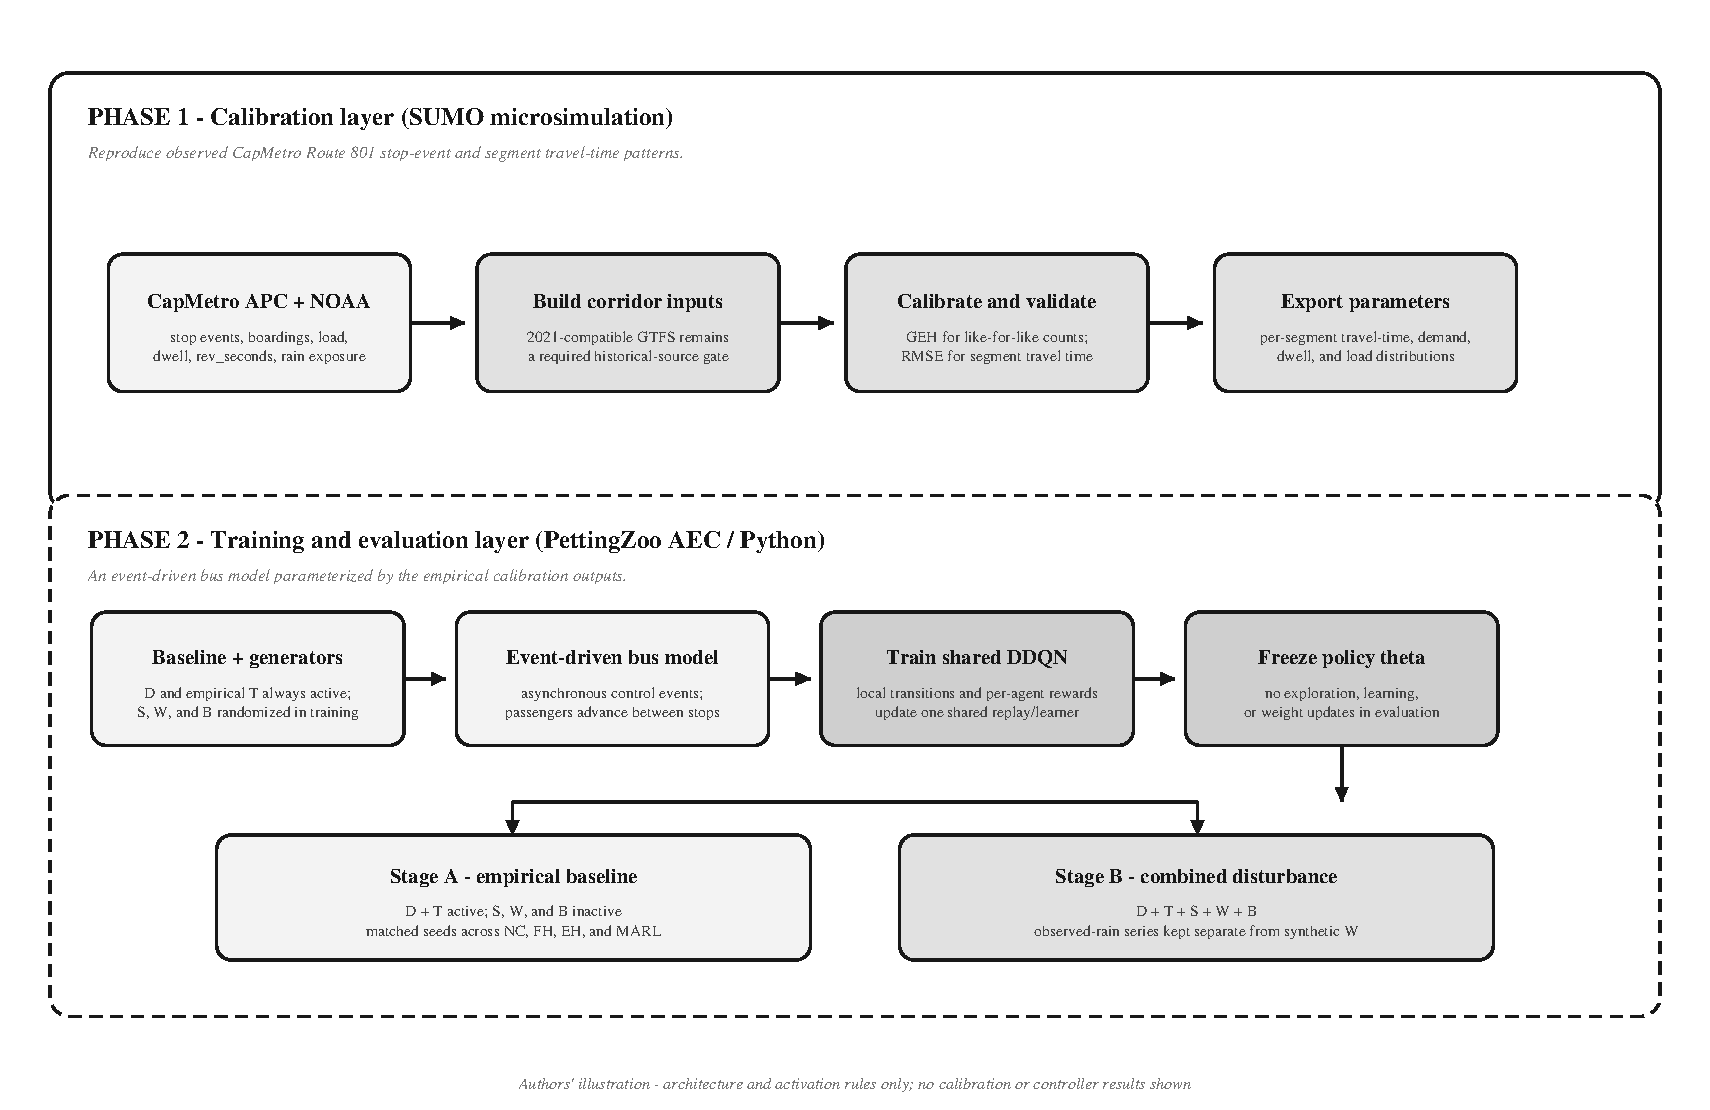
\includegraphics[width=\textwidth]{Figures/fig_3_1_pipeline (2).pdf}
    \caption[Two-phase simulation pipeline]{The two-phase simulation architecture. Authors' illustration.}
    \label{fig:pipeline}
\end{figure}

SUMO is used for the calibration layer because it integrates with Python via the Traffic Control Interface (TraCI) and supports the GEH and RMSE validation protocols described later in this section. Ollero et al.~\cite{Ollero2024EDSA} previously developed an AIMSUN microsimulation of the EDSA Busway corridor; this study implements an equivalent network in SUMO to take advantage of its open-source TraCI interface, while adopting the same calibration targets.


A pure-Python alternative without SUMO calibration was also considered but rejected: it would lack the empirically grounded per-segment travel-time distributions that the GEH-and-RMSE-calibrated SUMO model provides. The chosen approach uses each tool where it is strongest: SUMO for calibrated microscopic realism during the one-time calibration phase, and Python for fast event-driven Monte Carlo during training and evaluation. This keeps the experiment tractable on accessible hardware, including a single cloud-notebook GPU runtime. Rodriguez et al.~\cite{Rodriguez2023Cooperative} and Wang and Sun~\cite{Wangsun} adopt the same two-layer approach, using event-based custom simulators with calibration parameters supplied from empirical data.



As shown in Figure~\ref{fig:pipeline}, the pipeline proceeds in two phases. First, SUMO is calibrated against empirical bus data, and the resulting per-segment travel time, demand, and dwell time distributions are saved. Second, the Python environment loads these distributions and runs a lightweight event-based bus simulator for MARL training and evaluation. Because the Python environment draws from distributions extracted from the calibrated SUMO model, its statistical behavior matches SUMO at the level of per-segment travel time, demand, and dwell time. It does not reproduce SUMO's microscopic vehicle-to-vehicle interactions, but those interactions affect the reward function only through their aggregate effect on inter-stop bus travel time, which the calibrated distributions already capture. Rodriguez et al.~\cite{Rodriguez2023Cooperative} make the same argument: they trained in an event-based mesoscopic simulator parameterized by empirical corridor data.

\subsection{Control-Stop Selection}
\label{subsec:control-stop-selection}

The study operates on a sub-corridor of the EDSA Carousel route. Within the chosen sub-corridor, only a subset of stops is designated as \textit{control stops} where MARL agents are permitted to act; the remainder are non-control stops that contribute stochastic dwell and delay behavior without agent intervention. Control stops are selected according to four criteria, following Rodriguez et al.~\cite{Rodriguez2023Cooperative} and the minimal-intervention principle of Wang and Sun~\cite{Wangsun}:

\begin{enumerate}
    \item \textbf{Origin terminal.} The route origin is always a control stop, since it is the natural point at which initial headways are set before buses enter the corridor.
    \item \textbf{Onset of high-demand segments.} The first stop of each high-demand segment is designated a control stop, so that the agent can act before demand-driven irregularity propagates downstream.
    \item \textbf{Low through-volume preference.} Stops with substantial through-passenger volume (many onboard riders not alighting) are \textit{avoided} as control stops, so that holding actions do not penalize large numbers of passengers already in transit.
    \item \textbf{No adjacent control hubs.} Where two high-demand hubs are adjacent, only the upstream hub is designated, so that holding penalties do not compound across two consecutive control actions.
\end{enumerate}

These criteria are data-driven: they specify \textit{how} stops are selected from demand and through-volume statistics, without assuming which stops a particular dataset will yield. Once the operational data are processed (Section~\ref{subsec:data-pipeline}) and the per-stop demand and through-volume profiles are known, the criteria are applied to produce the control-stop list for the study sub-corridor.

\subsection{Environment Model Validation}

Before MARL training begins, the SUMO calibration layer is statistically verified to approximate real-world bus operation along the corridor. Two industry-standard calibration metrics are used: the GEH statistic for bus volume on the dedicated corridor, and the Root Mean Square Error (RMSE) for bus speed trajectories. The calibration is restricted to the bus corridor itself, since the agents' state and reward depend only on bus dynamics; surrounding mixed-traffic flows do not enter the Python environment. This GEH/RMSE procedure calibrates EDSA-specific parameters directly from EDSA operational data and does not depend on the North Luzon Expressway rainfall-impact figures cited as motivating evidence in Section~1.1 \cite{TSSP_Rain2018}; that citation establishes only that weather materially affects Philippine road-traffic operations in general, not any EDSA-specific speed or capacity value used in this calibration.

\begin{figure}[htbp]
    \centering
    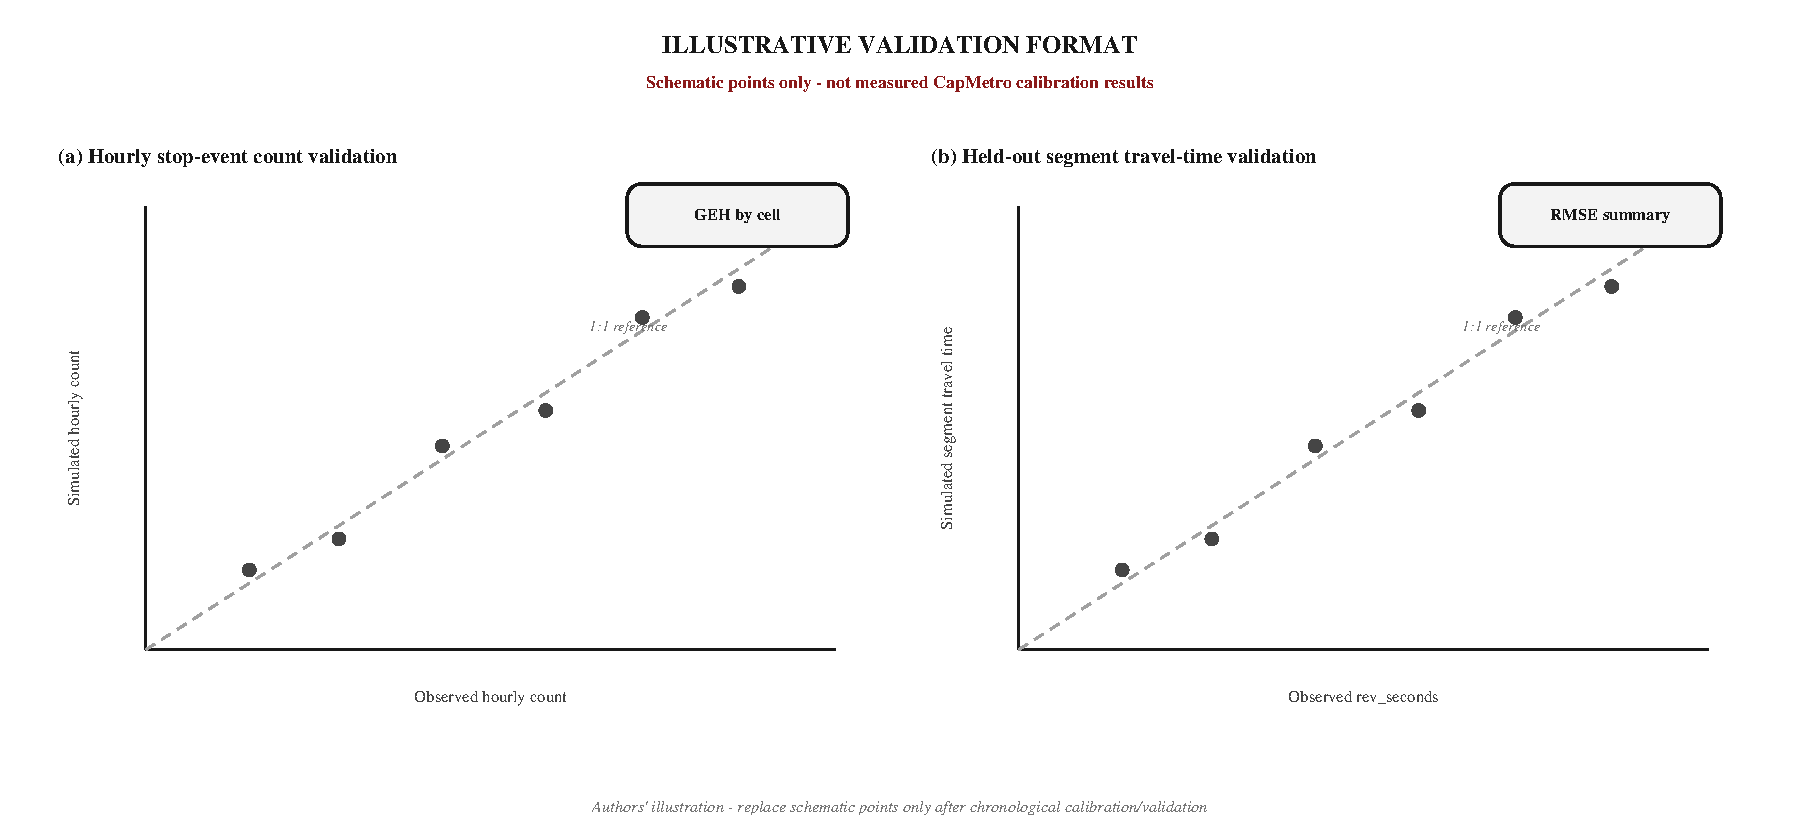
\includegraphics[width=\textwidth]{Figures/meth_fig_eo1_1_calibration (2).pdf}
    \caption[Illustrative SUMO calibration output]{Illustrative format of the
    SUMO calibration output. (a) Per-segment GEH statistic against the FHWA
    acceptance threshold of $\mathrm{GEH} < 5$; the corridor is accepted when at
    least 85\% of segments fall below the line. (b) Simulated bus-speed
    trajectory against the empirical observation used in the RMSE minimization
    step. Values shown are illustrative only. Authors' illustration.}
    \label{fig:calibration-illustrative}
\end{figure}

\subsubsection{Bus Volume Validation via GEH Statistic}

The GEH statistic, introduced for traffic-modelling acceptance testing in the UK Design Manual for Roads and Bridges \cite{DMRBV12}, measures the discrepancy between simulated and observed hourly bus volumes on individual corridor segments, illustrated in panel (a) of Figure~\ref{fig:calibration-illustrative}:

\begin{equation} GEH = \sqrt{\frac{2(M - C)^2}{M + C}} \label{eq:geh} \end{equation}

where $M$ is the hourly bus volume from the simulation and $C$ is the observed hourly bus count from empirical operational data. The environment is accepted when $GEH < 5$ for more than 85\% of corridor segments, following the FHWA Traffic Analysis Toolbox calibration criterion~\cite{FHWA2019TAT} as applied in recent SUMO calibration work by Patil et al.~\cite{Patil2025Conformal}.

\subsubsection{Speed Trajectory Calibration via RMSE}

Volume calibration alone does not guarantee that buses move realistically. RMSE evaluates how closely simulated bus speed trajectories match empirical observations, illustrated in panel (b) of Figure~\ref{fig:calibration-illustrative}:

\begin{equation} RMSE = \sqrt{\frac{\sum_{i=1}^{n}(x_{obs} - x_{model})^2}{n}} \label{eq:rmse} \end{equation}

where $x_{obs}$ is the observed bus speed and $x_{model}$ is the simulated bus speed \cite{Ollero2024EDSA}. To minimize RMSE, microscopic SUMO parameters like maximum desired speed and speed acceptance for the bus vehicle class are iteratively tuned to fit empirical speed profiles \cite{Ollero2024EDSA}. Once both the GEH threshold and RMSE minimization are achieved, the environment is treated as a validated representation of the operational scope.

\subsubsection{Real-Time Data Incorporation}

In a real-world deployment, the agent's state vector at each control event would be drawn from existing transit-data infrastructure: forward and backward headways $(h^-, \hat{h}^+)$ from Automatic Vehicle Location (AVL) feeds; onboard and waiting passenger counts from Automatic Passenger Counters (APC) and Automatic Fare Collection (AFC) terminals; and environmental flags from public weather APIs and incident-management systems \cite{Wangsun}. Within this study, the Python environment generates synthetic equivalents of these signals at each control event by querying the analytical bus model and combining outputs from the stochastic generators described below.

\subsection{Operating Conditions}

The study \textbf{evaluates} controllers under two distinct operating conditions. These conditions govern \textbf{evaluation only}; as detailed in the Training Protocol, the MARL policy is always trained with the full disturbance set active (domain randomization), and the two conditions below differ only in which disturbances are switched on when measuring the frozen, already-trained policy. The symbols used to define these conditions ($\eta$, $\sigma_d$, $\sigma_s$, and the breakdown rate $\lambda$) are collected in Table~\ref{tab:notation}.

\textbf{Ideal conditions.} The corridor operates under the empirical baseline from the operational dataset, with no additional disturbance. The weather disturbance generator is disabled ($\eta = 0$), the breakdown generator is disabled ($\lambda = 0$), and the demand and traffic-speed scaling factors are at their baseline means ($\sigma_d = 0$, $\sigma_s = 0$). Each bus therefore encounters the empirical mean travel time and demand profile for its segment and time of day. The Python environment still injects normal day-to-day variability through the calibrated per-segment distributions, so the ideal condition is \textit{stochastic but not disturbed} which comparable to a normal weekday with no incidents, severe weather, or surge events. This serves as the control condition for Stage A \textit{evaluation}; it is not a training setting, since training always exposes the policy to the full disturbance range.

\textbf{Non-ideal conditions.} One or more of the four stochastic generators described in the next section is activated. The full non-ideal evaluation (Stage B) sweeps the weather disturbance intensity $\eta$ across five values, with the breakdown generator active alongside throughout. Demand scaling remains active under both conditions to preserve realistic passenger-arrival variability. The traffic-speed generator governs inter-stop travel-time variability under the ideal condition; under the non-ideal condition, the heavier-tailed weather generator replaces it as the source of travel-time stochasticity, since its coefficient of variation $\eta \geq 0.3$ already spans and exceeds the variability range that the traffic-speed scaling produces (Section~\ref{subsec:stochastic-vars}). The two conditions therefore differ in which generator governs travel-time stochasticity and in whether the discrete breakdown generator is enabled.

Both conditions draw inter-stop travel time from distributions anchored to the same per-segment empirical baseline mean $\mu$ extracted during SUMO calibration; only the shape of variability changes between conditions. The non-ideal condition recovers the ideal condition as $\eta \to 0$, because the lognormal collapses to a point mass at $\mu$ when its coefficient of variation is zero. Performance differences between the two conditions therefore reflect a change in the variability profile of travel time, not a change in its mean or in the underlying network geometry.

Throughout this chapter, \textit{ideal conditions} and \textit{non-ideal conditions} refer to these operating states of the simulated environment. \textit{Baseline controllers} refers separately to the three non-MARL control strategies (No Control, Forward Headway, Even Headway) against which the MARL policy is benchmarked. A condition is a state of the world; a controller is a choice of algorithm.

\begin{table}[htbp]
\centering
\caption{Simulation parameter summary: fixed, swept/variable, and derived parameters.}
\label{tab:sim-parameters}
\small
\renewcommand{\arraystretch}{1.25}

\begin{tabularx}{\textwidth}{
>{\RaggedRight\arraybackslash}p{0.24\textwidth}
>{\RaggedRight\arraybackslash}p{0.09\textwidth}
X
>{\RaggedRight\arraybackslash}p{0.20\textwidth}
}

\toprule
\textbf{Parameter} & \textbf{Symbol} & \textbf{Value / Range} & \textbf{Source} \\
\midrule
\multicolumn{4}{l}{\textit{Fixed simulation parameters}} \\
\midrule

Simulation horizon & --- & Single simulated operating day (\%TODO-VAL: exact start/end hours) & Section~3.1 \\
Total stop count (sub-corridor) & $M$ & 24 & Introduction, Section~1.2.2 \\
Fleet size (active buses) & $N$ & $\approx 12$--$30$ & Introduction, Section~1.2.2 \\
Control stop count & --- & \%TODO-VAL: determined by criteria in Section~3.2.2 once dataset is processed & Section~3.2.2 \\
Scheduled headway & $H_0$ & \%TODO-VAL: from DOTr schedule records & DOTr records \\
Bus passenger capacity & --- & \%TODO-VAL: from DOTr fleet specification & DOTr records \\
Maximum holding duration & $\Delta T$ & \%TODO-VAL: to be set during implementation & Section~3.2.7 (Action Space) \\
Holding action bins & $\Omega$ & $\{0.0, 0.1, 0.2, 0.3, 0.4\}$ & Section~3.2.7 (Action Space) \\
Action space size per agent & $|A_i|$ & 10 (5 hold $\times$ 2 skip) & Section~3.2.7 (Action Space) \\
Monte Carlo runs per cell & $N_{\text{runs}}$ & $\geq 30$ & Section~3.1 \\
Discount / event-based discount & $\gamma$, $\beta$ & \%TODO-VAL: tuned during implementation & Section~3.2.7 \\

\midrule
\multicolumn{4}{l}{\textit{Swept / variable parameters}} \\
\midrule

Weather disturbance intensity & $\eta$ & $\{0.0, 0.3, 0.6, 1.0, 1.3\}$ & Section~3.2.6 \\
Demand scaling std.\ dev.\ (clip) & $\sigma_d$ & Clip $[1, 3]$ & Section~3.2.6 \\
Traffic-speed scaling std.\ dev.\ (clip) & $\sigma_s$ & Clip $[0.8, 1.2]$ & Section~3.2.6 \\
Breakdown rate & $\lambda$ & \%TODO-VAL: calibrated during implementation (events/hour) & Section~3.2.6 \\

\midrule
\multicolumn{4}{l}{\textit{Derived parameters (from SUMO calibration)}} \\
\midrule

Baseline inter-stop travel time & $\mu$ & Per-segment, per-time-of-day bin, \%TODO-DATA & SafeTravelPH dataset \\
Baseline travel-time std.\ dev.\ & $\sigma$ & Per-segment, per-time-of-day bin, \%TODO-DATA & SafeTravelPH dataset \\
Baseline coefficient of variation & $CV_0$ & $\sigma/\mu$ per segment, \%TODO-DATA & Computed from dataset \\
Lognormal shape parameter & $\sigma_{ln}$ & $\sqrt{\ln(\eta^2+1)}$ (Eq.~\ref{eq:sigma_ln}) & Method of moments \\
Lognormal location parameter & $\mu_{ln}$ & $\ln(\mu) - \sigma_{ln}^2/2$ (Eq.~\ref{eq:mu_ln}) & Method of moments \\

\bottomrule
\end{tabularx}
\end{table}

Table~\ref{tab:sim-parameters} therefore serves as the single reference point for every parameter used across this chapter. Parameters marked \%TODO-VAL are to be confirmed during the implementation phase upon receipt of the operational dataset and DOTr schedule records; parameters marked \%TODO-DATA will be computed during the SUMO calibration phase described in Section~3.2.3. The stop count ($M=24$) and fleet-size range ($N \approx 12$--$30$) are carried over from the state-space dimensionality discussion in Section~1.2.2 and are not new values introduced here.

\subsection{Data Processing}

The MARL framework is trained and evaluated on a single stream of input data pre-processed before training: corridor operational data used to calibrate SUMO and to derive baseline parameters for the stochastic generators. A second stream, the synthetic state observations generated by the Python environment at runtime, is produced on-the-fly during training and consumed once per control event.

\subsubsection{Required Datasets}

\begin{itemize}

\item \textbf{Corridor bus operational data.} A per-trip record of EDSA Carousel bus operation along the study sub-corridor, collected over a continuous observation window of at least two weeks. The required fields are GPS-tracked vehicle location, boarding and alighting events, passenger occupancy, operating speed, and \textit{dwell time} at each stop, the dwell time being the interval a bus spends stationary at a stop serving passengers, measured from the moment the doors open to the moment they close and the bus is ready to depart, exclusive of any holding time subsequently imposed by the controller. These records yield the empirical distributions of bus cruising speed, inter-stop travel time, and demand under ideal operating conditions, used both to calibrate SUMO and to define the baseline operating point of the stochastic generators. The baseline operating point for this study is established from a crowdsourced operational record collected from the EDSA Busway during July 2023 through the SafeTravelPH mobile application.

%A crowdsourced operational dataset of this form, for example, data collected from the EDSA Busway via the SafeTravelPH mobile application, provides a representative model of the required structure. Should bus-volume coverage prove insufficient for the GEH validation step, supplementary records may be requested from MMDA, DOTr, or the involved bus operators under the Freedom of Information process.

\end{itemize}

Table~\ref{tab:field-mapping} maps each required raw field to the parameter derived from it and the MARL component that parameter feeds into, connecting the data requirements above to the disturbance generators (Section~\ref{subsec:stochastic-vars}), the control-stop selection criteria (Section~\ref{subsec:control-stop-selection}), and the agent observation vector (Section~\ref{subsec:state-space}). The mapping reflects the study's design intent, not properties of a processed dataset; specific statistics remain \%TODO-DATA pending dataset acquisition.

\begin{table}[htbp]
\centering
\caption{Mapping of required raw dataset fields to derived parameters and their role in the MARL formulation.}
\label{tab:field-mapping}
\small
\renewcommand{\arraystretch}{1.25}

\begin{tabularx}{\textwidth}{
>{\RaggedRight\arraybackslash}p{0.19\textwidth}
>{\RaggedRight\arraybackslash}p{0.28\textwidth}
>{\RaggedRight\arraybackslash}X
}

\toprule
\textbf{Raw Field} & \textbf{Derived Parameter} & \textbf{MARL Component} \\
\midrule

GPS-tracked vehicle location &
Per-segment inter-stop travel time distribution ($\mu$, $\sigma$) &
SUMO speed calibration (RMSE, Section~\ref{subsec:stochastic-vars}); anchors the traffic-speed generator ($\sigma_s$) and the weather generator's baseline mean ($\mu$) \\

Boarding events &
Per-(stop, time-of-day) baseline demand rate &
Demand surge generator baseline ($\sigma_d$); waiting-passenger-count feature in the agent's local observation \\

Alighting events &
Through-passenger volume per stop &
Control-stop selection criterion 3 (low through-volume preference, Section~\ref{subsec:control-stop-selection}) \\

Passenger occupancy &
Per-segment load profile &
Onboard-passenger-count feature in the agent's local observation; dwell-time estimation \\

Operating speed &
Per-segment baseline cruising speed &
SUMO bus-volume calibration (GEH); traffic-speed generator baseline ($\sigma_s$) \\

Dwell time &
Per-(stop, time-of-day) dwell time distribution &
Event-driven bus model, used between control events to advance the simulation clock \\

\bottomrule
\end{tabularx}
\end{table}

Severe-weather conditions are not estimated from operational data in this study but are injected as a controlled experimental variable, with disturbance magnitudes anchored to validated literature values rather than to a corridor-specific severe-weather sample.

A short empirical observation window cannot reliably resolve the variance of a heavy-tailed severe-weather distribution at per-segment granularity, and a swept-disturbance design characterizes controller performance across a range of conditions rather than at a single uncertain calibration point. Because the disturbance conditions are random by construction, they are not drawn from any single fixed dataset: each Monte Carlo run generates a fresh, independently seeded realization of demand, traffic-speed, weather, and breakdown disturbances. The single empirical dataset is required only to fix the \textit{baseline} (ideal-condition) operating point against which these random disturbances are layered; the held-out validation split (Stage 3 below) confirms that the calibrated baseline generalizes beyond the records used to tune it. The full disturbance parameterization is described in Section~\ref{subsec:stochastic-vars}.

\subsubsection{Data Pre-Processing Pipeline}
\label{subsec:data-pipeline}

Pre-processing proceeds in three stages.

\textit{Stage 1: Cleaning.} Trip records with missing GPS coordinates, missing timestamps, negative inter-stop times, or trips that fail integrity checks (for example, a later stop served before an earlier one) are dropped. Remaining records are normalized to a common time zone. Because the operational observation window is short (on the order of two weeks), the data cannot support separate weekend or holiday demand profiles --- a window of this length yields too few weekend days and typically no holidays to estimate distinct calendars reliably. Records are therefore filtered to regular weekdays and binned by time-of-day, which is the calendar dimension that drives demand and travel-time variation within the modeled operating day. The restriction to weekday operation is recorded as a scope limitation.

\textit{Stage 2: Empirical distribution extraction.} For each (segment, time-of-day) bin, the cleaned operational data yield the mean $\mu$ and standard deviation $\sigma$ of inter-stop travel time under baseline operating conditions, producing the baseline coefficient of variation $CV_0 = \sigma / \mu$ used to anchor the disturbance generators. Boarding and alighting counts per (stop, time-of-day) bin yield the baseline demand profile. These statistics are serialized to disk as parameter files that the Python environment loads at initialization.

\textit{Stage 3: Train/validation split for calibration.} The calibration data are split chronologically into a calibration set, used to tune SUMO parameters until the GEH and RMSE targets are met, and a held-out validation set, used to confirm that the calibrated environment generalizes beyond the tuning data.

The MARL agents are not trained on these raw datasets directly. They are trained on synthetic state vectors $s_{i,t}$ produced by the Python environment at each control event. Each $s_{i,t}$ is assembled at runtime by querying the analytical bus model and is consumed once by the policy network before being discarded. There is no persistent training dataset of state-action transitions on disk other than the standard replay buffer used by the learning algorithm.

\subsection{Stochastic Disturbance Generators}
\label{subsec:stochastic-vars}

\paragraph{Disturbance Classes and Independence}

This study distinguishes five disturbance classes, denoted D, S, T, W, and B:

\begin{itemize}
\item \textbf{Stochastic demand (D):} the baseline, always-present day-to-day randomness in passenger arrivals, drawn from the calibrated per-(stop, time-of-day) demand distributions (Section~\ref{subsec:data-pipeline}). D is not a disturbance layered on top of a deterministic baseline; it \textit{is} the baseline stochastic environment, present in every run regardless of which other generators are active.
\item \textbf{Demand surge (S):} an episode-level multiplicative scaling factor, with standard deviation $\sigma_d$ (Table~\ref{tab:notation}), that amplifies baseline boarding rates above their empirical mean. S is the controlled experimental variable; D is always present, and S is what is added on top of it. Setting $\sigma_d = 0$ removes the surge and leaves only baseline demand variability (D).
\item \textbf{Traffic-speed perturbation (T):} an episode-level scaling of corridor cruising speed, with standard deviation $\sigma_s$, representing everyday congestion friction. T governs inter-stop travel-time variability under ideal conditions.
\item \textbf{Weather-induced delay (W):} a per-segment travel-time distribution with coefficient of variation $\eta$, drawn from a right-skewed lognormal rather than the Gaussian-based scaling used by T. W replaces T as the source of travel-time stochasticity once $\eta > 0$ (Section~\ref{subsec:stochastic-vars}).
\item \textbf{Discrete bus breakdown (B):} a Poisson-distributed discrete event, with rate $\lambda$, that permanently removes one bus from the active agent set for the remainder of the simulated day.
\end{itemize}

The four generators that produce S, T, W, and B are injected independently: no causal chain links them within the simulation. A breakdown event (B) does not trigger a demand surge (S) or a weather delay (W), and a weather event does not induce a mechanical failure. In practice, some real-world disturbances co-occur causally --- for example, heavy rain may both slow buses (W) and concentrate passengers at covered stops (S) --- but this study treats each generator as an independent factor. This design choice isolates the individual and combined effect of each disturbance class on controller performance and allows the single-disturbance ablation (Section~\ref{subsec:evaluation}) to attribute degradation unambiguously to a specific class.

Four stochastic generators inject variability into the Python environment. Generators (i) and (ii) follow the perturbation framework of Wang and Sun~\cite{Wangsun}; the weather generator's heavy-tailed lognormal formulation follows Patil et al.~\cite{Patil2025Conformal}; the breakdown generator follows the rescheduling formulation of Cao et al.~\cite{Cao2022Train}. Table~\ref{tab:notation} collects the symbols used across this section and the MARL formulation that follows.


\begin{table}[htbp]
\centering
\caption{Notation used in the stochastic generators and the MARL formulation.}
\label{tab:notation}

\small
\renewcommand{\arraystretch}{1.25}

\begin{tabularx}{\textwidth}{
>{\RaggedRight\arraybackslash}p{0.14\textwidth}
>{\RaggedRight\arraybackslash}X
>{\RaggedRight\arraybackslash}p{0.18\textwidth}
}

\toprule
\textbf{Symbol} & \textbf{Definition} & \textbf{Domain / units} \\
\midrule

$\eta$ &
Weather disturbance intensity; directly sets the coefficient of variation of disturbed inter-stop travel time ($CV=\eta$). $\eta=0$ disables the weather generator. &
dimensionless \\

$\sigma_d$ &
Standard deviation of the per-episode passenger-demand scaling factor. $\sigma_d=0$ fixes demand at its baseline mean. &
dimensionless \\

$\sigma_s$ &
Standard deviation of the per-episode traffic-speed scaling factor. $\sigma_s=0$ fixes cruising speed at its baseline mean. &
dimensionless \\

$\lambda$ &
Rate parameter of the Poisson process governing bus breakdowns. $\lambda=0$ disables breakdowns. &
events/hour \\

$\mu$ &
Baseline (empirical) mean inter-stop travel time for a given segment and time-of-day bin. &
seconds \\

$\sigma$ &
Baseline standard deviation of inter-stop travel time. &
seconds \\

$CV_0$ &
Baseline coefficient of variation, $CV_0=\sigma/\mu$, used to anchor the disturbance generators. &
dimensionless \\

$\mu_{ln},\sigma_{ln}$ &
Location and shape parameters of the lognormal weather-delay distribution (method-of-moments). &
--- \\

$h^-,\hat{h}^+$ &
Forward headway (gap to bus ahead) and estimated backward headway (gap to bus behind). &
seconds \\

$H_0$ &
Desired (scheduled) headway. &
seconds \\

$\alpha_{i,t}$ &
Holding-strength action of agent $i$, $\alpha_{i,t}\in\Omega=\{0.0,0.1,0.2,0.3,0.4\}$, scaled by $\Delta T$. &
dimensionless \\

$\Delta T$ &
Maximum holding duration that $\alpha_{i,t}$ scales. &
seconds \\

$\gamma,\beta$ &
Discount factor and event-based discount rate ($e^{-\beta t}$ replaces $\gamma$ for random inter-event times). &
dimensionless \\

$\theta$ &
Weights (parameters) of the online neural network (shared policy). &
dimensionless \\

$\theta^-$ &
Weights (parameters) of the target neural network in DDQN. &
dimensionless \\

$N$ &
Number of bus agents (also used for the Monte Carlo run count, $N\geq30$, where noted). &
count \\

\bottomrule
\end{tabularx}
\end{table}

\subsubsection{Random Seed Control}

All four generators draw from a single seeded pseudo-random number stream maintained by the Python NumPy library. At the start of each Monte Carlo run, a master seed is set in the simulation driver script, which initializes NumPy's BitGenerator. For each (disturbance level, control strategy) cell, the list of $N \geq 30$ seeds is fixed in advance and stored as a configuration file in the project repository. Within a disturbance level, the same seed list is reused across all four control strategies, so the demand trace, disturbance realization, and breakdown timing for run $k$ are identical regardless of which controller is active. This matching enables paired statistical comparisons: any difference in performance metrics between two controllers on run $k$ is attributable to the controller rather than to the disturbance realization \cite{Henderson2018Matters}. Seeds across runs are independent, and the choice $N \geq 30$ ensures that the Central Limit Theorem applies to the run-mean of each response variable. %For settings with heavy-tailed disturbances, bootstrap-based confidence intervals are reported rather than relying solely on the normal approximation at $N = 30$ \cite{Agarwal2021Precipice}.

\subsubsection{Passenger Demand}

The baseline empirical transit demand is perturbed each episode by a scaling factor sampled from $\mathcal{N}(1, \sigma_d^2)$ and clipped to $[1, 3]$, following the general Gaussian-clipped demand-scaling mechanism of Wang and Sun~\cite{Wangsun}, though this study adopts a narrower clip than their $[1, 10]$ range. The asymmetric clip focuses the test on demand surges rather than symmetric variation, since demand drops produce lightly loaded conditions that do not stress-test the controller. The upper bound of 3, corresponding to roughly a tripling of baseline boarding rates, is this study's own choice (\%TODO-VAL: revisit against Wang and Sun's wider range during implementation) rather than a value drawn from prior work. Sampling occurs at the start of each simulation run, producing varied demand profiles across episodes. In implementation, the scaling factor $f_d \sim \mathcal{N}(1, \sigma_d^2)$ is sampled once per episode at initialization and applied uniformly to every per-stop, per-time-of-day arrival rate for the duration of that simulated operating day, so all stops experience the same proportional demand shift within a single run while the shift itself varies across runs.

\subsubsection{Traffic Delays}

Mean cruising speed between stops is adjusted dynamically using a scaling factor drawn from $\mathcal{N}(1, \sigma_s^2)$, clipped to $[0.8, 1.2]$, representing typical daily congestion friction \cite{Wangsun}. In implementation, the speed scaling factor $f_s \sim \mathcal{N}(1, \sigma_s^2)$ is sampled once per episode and applied to the bus's mean cruising speed on every inter-stop segment traversal during that day, producing a uniformly slower or faster corridor for that run without segment-level variation beyond the calibrated baseline. This generator provides the baseline stochastic variability in inter-stop travel time when the weather generator is inactive. When the weather generator is active ($\eta > 0$), the heavier-tailed lognormal described below replaces this scaling as the source of travel-time variability: the lognormal coefficient of variation $\eta \geq 0.3$ used in the non-ideal sweep already exceeds the $\pm 20\%$ range that traffic-speed scaling produces, so the two generators do not compose on the same segment. The traffic-speed generator's empirical role persists through the per-segment baseline mean $\mu$ to which both generators are anchored.

\subsubsection{Weather-Induced Anomalies}

Severe-weather disturbances are injected as a controlled experimental variable rather than estimated from a fixed empirical sample.

The controlled variable in this generator is the coefficient of variation of inter-stop travel time, not a meteorological quantity. Severe weather is the motivating phenomenon, but the variable that enters the simulator and that the controller observes is the travel-time distribution itself. The lognormal is chosen to model the shape that any such heavy-tailed disruption produces on per-segment travel time, regardless of its meteorological label. In implementation, when $\eta > 0$ a fresh travel-time sample $T \sim \text{LogNormal}(\mu_{ln}, \sigma_{ln})$ is drawn independently for each bus at each inter-stop segment traversal during the episode, replacing the traffic-speed generator's output for that traversal; the lognormal parameters $\mu_{ln}$ and $\sigma_{ln}$ are computed from the segment's empirical mean $\mu$ and the swept $\eta$ via Equations~\eqref{eq:sigma_ln}--\eqref{eq:mu_ln}. The disturbance intensity sweep is therefore read as a span of travel-time variability magnitudes, not as a sweep across named weather categories.

Inter-stop travel time under disturbance is sampled from a Lognormal distribution, which captures the right-skewed, heavy-tailed delays observed in urban traffic under inclement weather \cite{Patil2025Conformal}. The lognormal is chosen over a Gaussian distribution, which is symmetric and cannot represent heavy right tails, and over Gamma or Weibull distributions, which can produce heavy tails but lack the direct empirical validation against urban traffic data that Patil et al.\ provide for the lognormal form. The distribution's mean is the baseline inter-stop travel time $\mu$ from the operational data, and its variability is set by a disturbance intensity parameter $\eta$, which directly specifies the coefficient of variation:

\begin{equation} CV = \eta \label{eq:cv_eta} \end{equation}

The lognormal shape and scale parameters follow the method-of-moments derivation:

\begin{equation} \sigma_{ln} = \sqrt{\ln(\eta^2 + 1)} \label{eq:sigma_ln} \end{equation}

\begin{equation} \mu_{ln} = \ln(\mu) - \frac{\sigma_{ln}^2}{2} \label{eq:mu_ln} \end{equation}

Travel time is drawn as $T \sim \text{LogNormal}(\mu_{ln}, \sigma_{ln})$. Patil et al.~\cite{Patil2025Conformal} tested this parameterization by generating SUMO-simulated travel times under the same CV-driven lognormal recipe --- with time windows and mean travel times anchored to INRIX historical data for an urban arterial corridor, not a freeway --- and confirming via the Kolmogorov-Smirnov test that the simulated distribution matches the assumed log-normal shape, reporting a close fit at the highest variability level they tested ($KS = 0.036$, $p = 0.94$ at $CV = 1.0$).

The disturbance intensity $\eta$ is swept across five values, $\eta \in \{0.0, 0.3, 0.6, 1.0, 1.3\}$, chosen to span and slightly exceed the empirically validated CV range of Patil et al.~\cite{Patil2025Conformal}, who evaluate scenarios at $CV \in \{0.1, 0.3, 0.5, 0.7, 1.0\}$. The basis for each swept value is as follows. $\eta = 0$ disables the generator and recovers the ideal condition. $\eta \in \{0.3, 0.6\}$ fall inside the validated range, representing moderate travel-time variability. $\eta = 1.0$ corresponds to the upper end of Patil et al.'s validated range and is adopted here as the nominal severe-disturbance operating point. $\eta = 1.3$ extends beyond the validated range as an extrapolated stress test; results at this level are interpreted as a probe of controller behavior under extreme conditions rather than as a calibrated scenario. Table~\ref{tab:eta-basis} summarizes this reasoning.

\begin{table}[htbp]
\centering
\caption{Basis for each swept weather-disturbance intensity value.}
\label{tab:eta-basis}
\small
\renewcommand{\arraystretch}{1.25}

\begin{tabularx}{\textwidth}{
>{\Centering\arraybackslash}p{0.08\textwidth}
X
}

\toprule
\textbf{$\eta$} & \textbf{Basis} \\
\midrule

0.0 & Generator off --- recovers the ideal baseline \\
0.3 & Inside Patil et al.'s validated range --- moderate variability \\
0.6 & Inside Patil et al.'s validated range --- moderate variability \\
1.0 & Top of Patil et al.'s validated range --- nominal severe operating point \\
1.3 & Beyond the validated range --- deliberate extrapolated stress test \\

\bottomrule
\end{tabularx}
\end{table}

The mapping from $\eta$ to a specific named weather severity (e.g.\ ``moderate rain'' versus ``typhoon-grade'') is not established by Patil et al., whose CV values are not labeled by weather category. The $\eta$ sweep should therefore be read as a span of travel-time variability magnitudes rather than as calibrated meteorological intensities. Reporting controller performance across this sweep characterizes degradation as a function of disturbance magnitude, which is methodologically stronger than evaluating at a single point.

\subsubsection{Bus Breakdowns}

Unlike the perturbations above, a bus breakdown is a \textit{discrete event} that removes a bus from active simulation \cite{Cao2022Train,Shi2022DistDRL}. Breakdowns are triggered at random times sampled from a Poisson process with a configurable rate $\lambda$ (Table~\ref{tab:notation}). In implementation, at each discrete simulation timestep of length $dt$, a Bernoulli trial with probability $\lambda \cdot dt$ is evaluated independently for each active bus; a success removes that bus from the active agent set for the remainder of the simulated day. When a breakdown occurs at bus $b_k$, $b_k$ is removed from the active agent set, leaving an enlarged headway between the trailing bus $b_{k-1}$ and the leading bus $b_{k+1}$. The passengers that $b_k$ would have served accumulate at the stops ahead of $b_{k-1}$, so the trailing bus inherits this residual demand as it advances.

A breakdown does not override any agent's policy; it changes the \textbf{state} the surviving agents observe and the \textbf{reward landscape} they face. The removal of $b_k$ is encoded in the downstream incident/breakdown flag of the trailing agent's observation (Section~\ref{subsec:state-space}), and the inherited residual demand sharply raises the headway-irregularity and dwell-time penalties that the trailing agent's reward already captures. Under these conditions, the stop-skipping action, which is part of the agent's normal action space (Section~\ref{subsec:action-space}) becomes strongly advantageous. Skipping a heavily loaded downstream stop lets $b_{k-1}$ shed onboard passengers (alighting permitted, boarding suppressed) and close the gap to $b_{k+1}$ before bunching sets in. The environment therefore \textit{induces} the recovery behavior through the state and reward signal, and the agent must \textit{learn} to select it; the action is never injected by the environment. This keeps the breakdown response consistent with decentralized execution and the Markov-game formulation, in which every action originates from $\pi_\theta$.

The Poisson assumption is a tractable approximation for the single-day simulation horizon, over which vehicle age, maintenance schedule, and mileage since last service can be treated as constant.


\subsection{MARL Architecture and MDP Formulation}

This subsection builds the formal learning framework in two steps. It first introduces the Bellman recursion that underlies value-based reinforcement learning, then specifies the Markov game tuple, the per-agent observation and action spaces, the reward-function design, and the proposed learning algorithm. The justification for choosing a multi-agent formulation over a single-agent alternative is presented in Chapter~1.

\subsubsection{Bellman Foundation}

At the core of reinforcement learning is the dynamic programming principle established by Bellman~\cite{Bellman1957}. The agent's objective is to maximize the expected sum of discounted future rewards. The state-action value function $Q^\pi(s,a)$, denoting the expected return from taking action $a$ in state $s$ and following policy $\pi$ thereafter, satisfies the Bellman optimality equation:

\begin{equation}
Q^*(s, a) = \mathbb{E} \left[ r(s, a) + \gamma \max_{a'} Q^*(s', a') \mid s, a \right]
\label{eq:bellman}
\end{equation}

where $s'$ is the state reached after applying action $a$, $r(s,a)$ is the immediate reward, and $\gamma \in [0, 1)$ is the discount factor. This equation is relevant here for two reasons. First, it shows that a long-horizon control policy can be learned by recursively backing up local one-step rewards, making it computationally feasible to evaluate the downstream effects of a holding or skipping decision without enumerating every future stop on the route. Second, in the asynchronous bus-control setting, the time between two consecutive control events is itself random. Following Bradtke and Duff~\cite{Bradtke1995}, the discount factor in Eq.~\eqref{eq:bellman} is replaced by an event-based discount $e^{-\beta t}$ that scales with the elapsed time between events. Each agent's learning target is therefore an event-adjusted version of Eq.~\eqref{eq:bellman}, not a fixed-tick MDP target. By convention throughout this chapter, $\gamma$ denotes the nominal discount factor as it appears in the canonical Bellman and DDQN equations, while $e^{-\beta t}$ is the event-based discount actually applied in the asynchronous setting; wherever $\gamma$ appears in a value-function equation, it is instantiated by $e^{-\beta t}$ at runtime.


\subsubsection{Markov Game Formulation}

Following Littman~\cite{Littman1994}, the bus fleet control problem is formulated as a multi-agent extension of a Markov Decision Process, a Markov game defined by the tuple $G = \langle N, S, A, P, R, \gamma \rangle$:

\begin{itemize}
\item $N$: number of bus agents.
\item $S$: joint state space.
\item $A$: joint action space.
\item $P$: state-transition function $P(s_{t+1}\mid s_t, a_t)$.
\item $R$: reward function.
\item $\gamma \in [0, 1)$: discount factor.
\end{itemize}

Because bus control is asynchronous and event-driven, agents act only upon arrival at a control stop. The formulation maintains a per-agent local transition $P_i : S_i \times A_i \rightarrow S_i$, with $S_i$ the local observation of agent $i$ \cite{Wangsun,Rodriguez2023Cooperative}.

\subsubsection{Agents ($N$)}

The decision-making agents are the individual bus units $i \in N$ operating along the corridor. To avoid combinatorial blow-up and to keep the system invariant to fleet size, all agents share a single neural-network policy under a \textbf{parameter-sharing} architecture and act on their own local observations at deployment \cite{Wangsun,Rodriguez2023Cooperative,Christianos2021PS}. Parameter sharing means that one set of network weights serves every bus; each bus computes its own action from its own observation, but learning updates from any bus improve the policy for all.

\subsubsection{State Space and Local Observations ($S_i$)}
\label{subsec:state-space}

The local observation $s_{i,t}$ at agent $i$ on arrival at a control stop is a vector composed of:

\begin{itemize}
\item \textbf{Spatial location:} index of the current control stop.
\item \textbf{System regularity:} forward headway $h^-$ and estimated backward headway $\hat{h}^+$, both available from AVL feeds in deployment \cite{Wangsun}.
\item \textbf{Passenger demand:} onboard passenger count and estimated number of passengers waiting at the stop, available from APC/AFC systems \cite{Wangsun}.
\item \textbf{Environmental flags:} encoded indicators for the current disturbance intensity and any active downstream incident or breakdown.
\end{itemize}

\begin{table}[htbp]
\centering
\caption{Agent observation vector: features, symbols, and data sources.}
\label{tab:observation-features}
\small
\renewcommand{\arraystretch}{1.25}

\begin{tabularx}{\textwidth}{
>{\RaggedRight\arraybackslash}p{0.24\textwidth}
>{\RaggedRight\arraybackslash}p{0.11\textwidth}
>{\RaggedRight\arraybackslash}X
>{\RaggedRight\arraybackslash}X
}

\toprule
\textbf{Feature} & \textbf{Symbol} & \textbf{Deployment Source} & \textbf{Simulation Source} \\
\midrule

Control stop index & --- & Route map (static) & Hardcoded stop list \\
Forward headway & $h^-$ & AVL feed & Event-driven bus model \\
Estimated backward headway & $\hat{h}^+$ & AVL feed & Event-driven bus model \\
Onboard passenger count & --- & APC system & Running tally in bus model \\
Waiting passenger count at stop & --- & AFC terminal / platform sensors & Stop queue in bus model \\
Disturbance intensity flag & $\eta$ (encoded) & Weather API / public incident alert & Active generator parameter \\
Downstream incident / breakdown flag & $b$ (binary) & Incident management system & Breakdown generator output \\

\bottomrule
\end{tabularx}
\end{table}

As Table~\ref{tab:observation-features} shows, in simulation all observation features are generated synthetically by the Python environment at each control event by querying the analytical bus model and the active stochastic generators; no real sensor data is consumed during training or evaluation.

\subsubsection{Action Space ($A_i$)}
\label{subsec:action-space}

The agent's action $a_{i,t} = \pi_\theta(s_{i,t})$ combines two discrete components, following Rodriguez et al.~\cite{Rodriguez2023Cooperative}:

\begin{itemize}
\item \textbf{Holding control:} a holding-strength parameter $\alpha_{i,t} \in \Omega = \{0.0, 0.1, 0.2, 0.3, 0.4\}$, multiplied by a maximum holding duration $\Delta T$ to yield seconds held; $\alpha_{i,t} = 0$ means no holding.
\item \textbf{Stop-skipping:} a binary decision to bypass the next stop, triggered when the bus is severely delayed and near capacity, allowing headway recovery. Skipping is disallowed at the origin terminal and is not permitted if the immediately preceding trip already skipped that stop, so no passenger is denied service twice in a row.
\end{itemize}

The full action set is the Cartesian product of these two components: $|A_i| = 5 \times 2 = 10$ discrete actions per control event, allowing the agent to select a holding strength and a skip decision independently at each control event. This is a broader action space than Rodriguez et al.~\cite{Rodriguez2023Cooperative}, whose combined holding-and-skipping controller (DDQN-HA) instead selects among six \textit{mutually exclusive} actions: five holding strengths $\Omega = \{0.0, 0.1, 0.2, 0.3, 0.4\}$ (with $\omega = 0$ already covering the no-holding case) plus a single skip action. The discretized holding-strength set $\Omega$ adopted here matches theirs exactly. A continuous holding parameter $\alpha \in [0, 1]$ was considered, following Wang and Sun~\cite{Wangsun}, but rejected for two reasons. First, continuous actions require actor-critic algorithms, whose training instability compounds across the swept-disturbance evaluation budget. Second, real driver compliance with holding instructions is itself imperfect: Rodriguez et al.~\cite{Rodriguez2023Cooperative} model non-compliant drivers as departing after only 60--80\% of the instructed holding time, so continuous precision in $\alpha$ is not meaningful at deployment.

\subsubsection{Reward Function ($R$) and Objective}
\label{subsec:reward}

The infinite-horizon objective of agent $i$ is the expected cumulative event-discounted return

\begin{equation}
R_i = \mathbb{E}\!\left[\sum_{k=0}^{\infty} e^{-\beta t_k}\, r_{i, t+k}\right],
\end{equation}

where $t_k$ is the elapsed time to the $k$-th future control event, consistent with the event-based discount introduced earlier.

The \textbf{structure} of the per-event reward $r_{i, t+k}$ --- its component terms and the operational priorities they encode --- is defined in this chapter. Its \textbf{exact weighting and sensitivity analysis} are a research objective of this study (Specific Objective 2, Expected Output 2.1), to be finalized during implementation rather than inherited from prior work. This separation is deliberate: the reward \textit{form} is grounded here, while the tuning of its coefficients is treated as an empirical question. The reward formulation must balance three competing operational priorities: (i) headway regularity, since bunching is the primary failure mode of bus corridors; (ii) passenger waiting time at served stops, which is the most direct passenger-experience metric; and (iii) a penalty term that discourages degenerate skipping behavior, since an unconstrained skip action could otherwise reduce headway variance by refusing to serve passengers. Existing MARL bus-control reward formulations span a range of trade-offs among these priorities, from headway-coefficient-of-variation forms for holding-only action spaces \cite{Wangsun,Wang2023MultiObj} to passenger-time forms for combined holding-and-skipping action spaces \cite{Rodriguez2023Cooperative}. This study establishes the overall reward structure for the hybrid action space by defining the three reward components and their additive formulation, while treating the corresponding weighting coefficients, together with their sensitivity analysis, as the implementation-phase deliverable under Expected Output 2.1. Although the component structure is fixed at this stage, the coefficients remain as placeholders to be determined during implementation through experimental evaluation.

The reward is computed independently for each agent at every control event rather than as a shared team-level objective. Accordingly, $r_{i,t}$ represents the reward assigned to agent $i$ and is stored as that agent's transition in the shared replay buffer (Training and Execution Protocol, step 4). Each bus is therefore evaluated based on the consequences of its own action, even though all agents learn from a common shared network. Since the reward is derived from locally observable quantities already contained in the agent's observation, particularly the forward and backward headway measurements, the resulting signal remains aligned with corridor-wide service regularity without requiring a centralized reward computation during execution.

The overall reward function is expressed as the weighted sum of three penalty terms:

\begin{equation}
r_{i,t+k} = -w_1 \cdot (\text{headway-irregularity term}) - w_2 \cdot (\text{waiting-time term}) - w_3 \cdot (\text{skip-degeneracy term}),
\label{eq:reward-form}
\end{equation}

where $w_1$, $w_2$, and $w_3$ denote the weighting coefficients (\%TODO-VAL) to be determined through the Expected Output 2.1 sensitivity analysis. Each component is formulated as a non-positive penalty, allowing the agent to maximize its cumulative return in Eq.~\eqref{eq:bellman} by minimizing headway irregularity, passenger waiting time, and unnecessary stop-skipping behavior. Consequently, this chapter establishes the reward formulation and its optimization objective, while the specific mathematical expressions and coefficient values are reserved for the implementation and evaluation phase.

\subsubsection{Proposed Learning Algorithm}
\label{subsec:proposed-algorithm}

The fully discrete action space ($|A_i| = 10$) makes value-based learning a natural fit. This study adopts \textbf{Double Deep Q-Network (DDQN)~\cite{vanHasselt2016DDQN} with parameter sharing under centralized training and decentralized execution (CTDE)}. CTDE means the policy is trained with access to information from all agents but each bus acts on its own local observation alone at deployment, so the trained system does not require a centralized real-time controller. The choice follows Rodriguez et al.~\cite{Rodriguez2023Cooperative}, who used the same DDQN-based framework for cooperative holding-and-skipping control on a comparable corridor.

DDQN is chosen over three categories of alternatives. \textit{Plain DQN}~\cite{Mnih2015DQN} overestimates Q-values in noisy environments \cite{vanHasselt2016DDQN,Henderson2018Matters}, which the high-variance disturbance regime in this study would amplify. DDQN's double estimator addresses this by decoupling action selection from evaluation \cite{vanHasselt2016DDQN}. \textit{Actor-critic methods such as MAPPO and MADDPG} are compatible with continuous action spaces but unnecessary given the discrete action-space decision above; they would also introduce training instability that compounds across the swept-disturbance evaluation budget. \textit{Distributional methods such as Wang and Sun's IQNC-M} \cite{Wangsun} model the full return distribution rather than its expectation and offer strong performance on this problem class, but their meta-learning training procedure adds implementation risk beyond the scope of a thesis-scale project; IQNC-M is noted as a comparison target for future work.

Two enhancements from the recent bus-control literature will be tested during implementation: extending agent awareness to include neighboring-trip information in the observation and reward, as in Rodriguez et al.'s DDQN-HA variant \cite{Rodriguez2023Cooperative}, and credit assignment via inductive graph learning, as in Wang and Sun's CAAC framework \cite{Wangsun}. The final architecture will be selected based on training stability and validation-set passenger waiting time after a fixed training budget.


\subsubsection{Double Deep Q-Network Foundation}
\label{subsec:ddqn-foundation}

The Bellman optimality equation defines the value $Q^*(s,a)$ that an ideal controller would assign to each state-action pair, but it cannot be solved exactly for a state space as large as the bus-control problem, where the observation is a continuous vector of headways, loads, and queues. Two approximations bridge this gap. $Q$-learning~\cite{Bellman1957,Littman1994} replaces the exact solution with an iterative update that nudges a stored estimate $Q(s,a)$ toward the one-step Bellman target $r + \gamma \max_{a'} Q(s',a')$ after each transition. The Deep $Q$-Network (DQN)~\cite{Mnih2015DQN} replaces the lookup table with a neural network $Q(s,a;\theta)$, so that the value function generalizes across the continuous state vectors the bus environment produces. DQN trains $\theta$ by minimizing the temporal-difference loss between the network's prediction and a target computed from a periodically frozen copy of the network, with transitions drawn from an experience replay buffer to decorrelate consecutive samples.

DQN has a known issue: it systematically overestimates action values~\cite{vanHasselt2016DDQN}. The cause is the single $\max$ operator in the target. Because the same network both selects the next action ($\arg\max_{a'}$) and evaluates it ($\max_{a'} Q$), noise in value estimates is amplified the $\max$ preferentially picks whichever action happens to be overvalued, and that inflated value propagates into the target. In a low-variance environment this bias is manageable, but the swept-disturbance regime in this study generates heavy-tailed returns that feed the overestimation mechanism directly.

The Double Deep $Q$-Network (DDQN)~\cite{vanHasselt2016DDQN} removes this bias by decoupling action selection from action evaluation. The online network (weights $\theta$) selects the next action, but a separate target network (weights $\theta^-$) evaluates that action's value:

\begin{equation}
y^{\text{DDQN}} = r(s,a) + \gamma\, Q\!\left(s',\, \arg\max_{a'} Q(s', a'; \theta);\; \theta^-\right),
\label{eq:ddqn_target}
\end{equation}

For the overestimation to persist, both networks would have to overvalue the same action simultaneously, which is less likely than a single network doing so alone. The network is trained by minimizing the squared temporal-difference error:

\begin{equation}
\mathcal{L}(\theta) = \mathbb{E}_{(s,a,r,s') \sim \mathcal{D}} \left[ \left( y^{\text{DDQN}} - Q(s,a;\theta) \right)^2 \right],
\label{eq:ddqn_loss}
\end{equation}

where $\mathcal{D}$ is the experience replay buffer and the target weights $\theta^-$ are held fixed for a number of updates (or slowly tracked toward $\theta$) so that the regression target does not shift at every step.

Three properties make DDQN appropriate for this study. First, the discrete action space ($|A_i| = 10$) is the setting value-based methods handle well: the $\arg\max$ in Eq.~\eqref{eq:ddqn_target} is a finite enumeration over ten options. Second, the double estimator addresses the overestimation that high-variance disturbance returns would otherwise amplify. Third, DDQN inherits DQN's experience-replay and target-network machinery, which provides sufficient training stability without the auxiliary mechanisms that actor-critic methods require; this point is discussed further in Section~\ref{sec:challenges}. The event-based discount $e^{-\beta t}$ replaces the fixed $\gamma$ in Eq.~\eqref{eq:ddqn_target} when the target is computed in the asynchronous setting, so the DDQN target inherits the same event-adjustment as the underlying Bellman recursion. The combination of DDQN with parameter sharing and the CTDE scheme is specified in the Proposed Learning Algorithm subsection.

\subsubsection{Training and Execution Protocol}

The learning process follows the standard reinforcement-learning feedback loop under the asynchronous, event-driven bus-control setting and the CTDE scheme described above, illustrated in Figure~\ref{fig:aec-training}. The loop, repeated at every control event during training, proceeds as follows:

\begin{enumerate}
\item \textbf{Observe.} When bus agent $i$ arrives at a control stop, the Python environment assembles its local observation $s_{i,t}$ (Section~\ref{subsec:state-space}) from the analytical bus model and the active stochastic generators.
\item \textbf{Act.} The shared policy network selects an action $a_{i,t}$ (holding strength and skip decision) from $s_{i,t}$ using an $\epsilon$-greedy rule over the estimated $Q$-values during training, and greedily ($\arg\max_a Q$) at evaluation.
\item \textbf{Transition and reward.} The environment applies $a_{i,t}$, advances the simulation to the next control event, and returns the event-discounted reward $r_{i,t}$ (Section~\ref{subsec:reward}).
\item \textbf{Store.} The transition $(s_{i,t}, a_{i,t}, r_{i,t}, s_{i,t'})$, where $t'$ is the agent's next control event, is written to a shared experience replay buffer common to all agents under parameter sharing.
\item \textbf{Update.} Mini-batches sampled from the replay buffer update the shared online network by minimizing the DDQN temporal-difference loss against a slowly-updated target network; experience from every bus updates the single shared parameter set.
\end{enumerate}

This loop is the feedback mechanism that distinguishes the learned controller from the fixed-rule baselines, which compute a holding time directly from the current headways with no update step.

The protocol is split into a training phase and an execution (evaluation) phase:

\begin{itemize}
\item \textbf{Centralized training phase.} The loop above is run for a fixed episode budget with the stochastic disturbance generators active, so that the policy encounters demand surges, traffic-speed friction, weather delays, and breakdowns during training. A policy that never sees a breakdown or heavy-tailed delay during learning has no basis for responding to one at deployment. This follows the domain-randomization approach of Tang et al.~\cite{Tang2024Curriculum}, who randomize demand and schedule variables during training to obtain policies that generalize to real-world traffic variability. Training uses system-wide information where it stabilizes learning (e.g.\ a shared reward and shared buffer), and experience from all buses contributes to one shared network.

\item \textbf{Decentralized execution phase.} The trained network's weights are frozen. During Monte Carlo evaluation (Stages A and B), each bus acts independently and greedily on its own local observation $s_{i,t}$ alone, with no centralized controller and no further weight updates. The fixed policy is evaluated across both the ideal condition (Stage A) and the swept non-ideal condition (Stage B), so that its behavior is measured on disturbance realizations it did not see during training but which are drawn from the same generative process.
\end{itemize}

\begin{figure}[htbp]
    \centering
    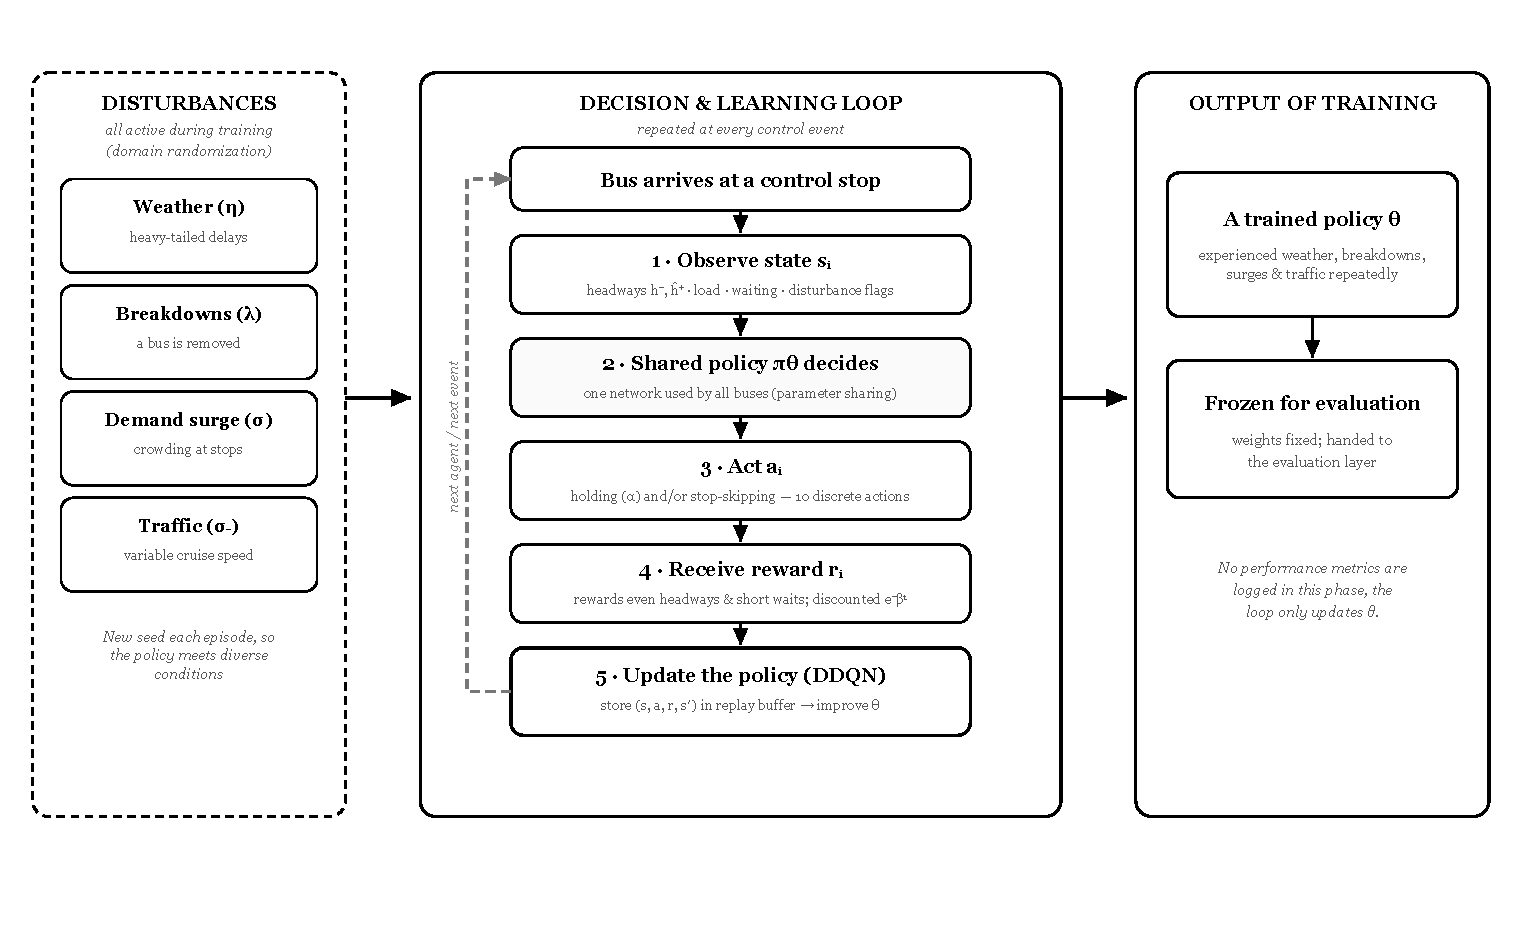
\includegraphics[width=\textwidth]{Figures/fig_3_2_aec_training.pdf}
    \caption[Agent--environment cycle (training)]{The asynchronous agent--environment
    cycle during training. Authors' illustration.}
    \label{fig:aec-training}
\end{figure}
 

Because heavy-tailed returns can destabilize value-based learning if injected without safeguards \cite{Henderson2018Matters,Agarwal2021Precipice}, training under disturbance is paired with the stabilizers discussed in Section~\ref{sec:challenges}: DDQN's double estimator, reward clipping, and slow target-network updates. If training under the full disturbance set proves unstable at the highest intensities despite these measures, a curriculum that ramps disturbance intensity over the course of training~\cite{Tang2024Curriculum} is retained as a fallback.

\clearpage

\subsection{Baseline Controllers for Comparison}

The MARL policy is benchmarked against three baseline controllers: \textbf{No Control (NC)}, \textbf{Forward Headway (FH)}, and \textbf{Even Headway (EH)}. These are the standard benchmark set in the MARL bus-control literature; both Wang and Sun \cite{Wangsun} and Rodriguez et al.~\cite{Rodriguez2023Cooperative} use this trio. Using the same baselines makes the results directly comparable to published work.

\subsubsection{No Control (NC)}

No holding or skipping is applied. Each bus dwells only for the time required to serve boarding and alighting passengers, then departs immediately. NC serves as the lower bound of the comparison: it isolates the natural corridor behavior without any regularization. If MARL cannot beat NC, the controller is doing more harm than good. NC also provides the reference point for measuring the severity of bus bunching. Under non-ideal conditions, NC has no corrective mechanism whatsoever, so demand surges, weather-induced delays, and breakdowns are expected to compound directly into bunching with no attenuation.

\subsubsection{Forward Headway (FH)}

The classical holding rule introduced by Daganzo~\cite{Daganzo2009}. When a bus arrives at a control stop, its holding time is:

\begin{equation}
d_{FH} = \max\!\left\{0,\, \bar{d} + g\,(H_0 - h^-)\right\}
\label{eq:fh}
\end{equation}

where $H_0$ is the desired (scheduled) headway, $h^-$ is the forward headway (time gap to the bus ahead), $\bar{d}$ is the average slack delay at equilibrium, and $g > 0$ is a control gain parameter. If a bus is running closer to the bus ahead than scheduled ($h^- < H_0$), it holds for an additional period proportional to the gap deficit; if it is already at or beyond the desired spacing ($h^- \geq H_0$), it does not hold. Parameters $\bar{d}$ and $g$ follow Daganzo's original values. FH represents local, single-agent reactive control: each bus reacts only to information about the bus immediately ahead. Because Eq.~\eqref{eq:fh} conditions only on $h^-$, FH is expected to partially correct demand- and traffic-induced bunching but to respond poorly to a breakdown: it has no observation of the enlarged gap a failed bus leaves for the bus behind it, so the trailing bus's holding decision is uninformed by the breakdown until the irregularity has already propagated back to it.

\subsubsection{Even Headway (EH)}

A more globally aware rule that holds buses to equalize the forward and backward gaps simultaneously, following Rodriguez et al.~\cite{Rodriguez2023Cooperative}:

\begin{equation}
T_{EH} = \max\!\left\{\min\!\left[\frac{\hat{h}^+ - h^-}{2},\; 0.4\,H_0\right],\, 0\right\}
\label{eq:eh}
\end{equation}

where $h^-$ is the forward headway, $\hat{h}^+$ is the estimated backward headway (time gap to the bus behind), and $\frac{\hat{h}^+ - h^-}{2}$ is the holding time that would split the difference evenly between the two gaps. The hold is capped at $0.4\,H_0$ (40\% of the scheduled headway), the bound Rodriguez et al.\ used to prevent excessive intervention. This cap matches the maximum value in the MARL action set $\Omega = \{0, 0.1, 0.2, 0.3, 0.4\}$, so EH and MARL are constrained to the same maximum hold and the comparison is fair. EH represents globally-aware reactive control: it uses information about both neighbors but follows a fixed rule rather than a learned policy. Because Eq.~\eqref{eq:eh} is a fixed linear rule computed from the currently observed gaps, EH is expected to handle breakdowns better than FH, since the enlarged backward gap $\hat{h}^+$ enters the rule directly, but it has no mechanism to anticipate or discount the heavier-tailed delays that the weather generator introduces, since the rule was not designed with a heavy-tailed disturbance in mind.
\clearpage
\subsubsection{Baseline Comparisons}

The three controllers span the comparison space. NC tests whether intervention helps at all. FH tests whether MARL outperforms classical local reactive control. EH tests whether MARL outperforms classical global reactive control and EH is the stronger of the two classical baselines, consistently reported as the best non-RL controller in the literature \cite{Wangsun,Rodriguez2023Cooperative}. The acceptance criterion for the MARL policy in Stage A (Section~\ref{subsec:evaluation}) is therefore stated relative to EH: matching or beating EH is the meaningful test.

This three-way comparison also allows the study to attribute MARL's advantage. If MARL beats NC but not FH or EH, the benefit is from intervening, not from learning. If MARL beats FH but not EH, the benefit is from global awareness, not from learning. Only if MARL beats EH does the benefit come from the learned policy itself. The same logic applies in Stage B: the disturbance-handling claim is meaningful only if MARL's advantage over EH grows with $\eta$, since both controllers see the same disturbance realizations.

State-of-the-art MARL methods such as CAAC and IQNC-M \cite{Wangsun} were considered as additional baselines but excluded. Including them would shift the research question from ``does MARL help on EDSA?'' to ``which MARL variant is best?'', a different question requiring different experimental data. 

\subsection{Data Analysis Methods}

The three response variables logged per run are defined as follows. \textbf{Mean passenger waiting time} ($\bar{W}$) is the average time elapsed from a passenger's arrival at a stop to their successful boarding, averaged across all passengers served and all stops over one simulated operating day:

\begin{equation}
\bar{W} = \frac{1}{P} \sum_{p=1}^{P} \left(t_p^{\text{board}} - t_p^{\text{arrive}}\right)
\label{eq:waiting_time}
\end{equation}

where $P$ is the total number of passengers served in the run and $t_p^{\text{board}}$, $t_p^{\text{arrive}}$ are the boarding and arrival times of passenger $p$. \textbf{Mean total travel time} ($\bar{T}$) is the average elapsed time from a bus's departure from the origin terminal to its arrival at the final stop of the sub-corridor, averaged across all bus trips completed during the simulated day. \textbf{Headway coefficient of variation} ($CV_h$) measures headway regularity:

\begin{equation}
CV_h = \frac{\sigma_h}{\mu_h}
\label{eq:headway_cv}
\end{equation}

where $\sigma_h$ and $\mu_h$ are the standard deviation and mean of observed inter-bus headways recorded at all stops over one simulated operating day. $CV_h = 0$ denotes perfectly regular headways; larger values indicate increasing bunching severity. This construction mirrors the baseline coefficient of variation $CV_0$ already defined for travel time (Table~\ref{tab:notation}), applied here to the headway distribution instead.

For each (control strategy, disturbance level) cell, $N \geq 30$ independent Monte Carlo runs are executed using matched random seeds across strategies. Three response variables are logged per run: mean passenger waiting time, mean total travel time, and headway coefficient of variation. The choice $N \geq 30$ ensures that the Central Limit Theorem applies to the run-mean of each response variable \cite{Wasserman2004}.

Statistical significance of performance differences between controllers will be assessed at a significance level of $\alpha = 0.05$. Because the same random seeds are reused across controllers within a disturbance level, comparisons between two controllers at the same disturbance level are naturally paired: the only difference between two runs is the controller, not the disturbance realization. Paired-sample tests will therefore be used for within-disturbance-level comparisons; unpaired tests will be used where seed matching does not apply (for example, comparing the same controller across different disturbance levels). Multiple-comparison correction will be applied across the four controllers to control the family-wise error rate.

For non-ideal disturbance levels, performance degradation is computed as the percentage change in each response variable relative to the same controller's $\eta = 0$ ideal-condition result. Confidence intervals on this degradation ratio will be computed by bootstrap resampling, since ratios of sample means are not guaranteed to be normally distributed and may be skewed under high-disturbance conditions \cite{EfronTibshirani1993}. The specific hypothesis tests, normality checks, multiple-comparison procedure, and bootstrap parameters will be selected during the implementation phase in consultation with the research supervisor, following recent guidance on reinforcement-learning evaluation~\cite{Henderson2018Matters,Agarwal2021Precipice}. Analysis is performed in Python using NumPy, SciPy, and pandas; raw run logs and analysis notebooks are version-controlled for reproducibility.

\subsection{Evaluation Methods}
\label{subsec:evaluation}



\textbf{Stage A: Ideal-condition evaluation.} The weather and breakdown generators are disabled; demand and traffic-speed scaling are fixed at baseline means ($\eta = 0$). The trained MARL policy and the three baselines are each run for $N \geq 30$ Monte Carlo iterations with matched seeds, reported in the format shown in Figure~\ref{fig:stage-a-illustrative}. Under ideal conditions EH is already near-optimal, so parity with EH is an acceptable Stage A outcome. Outperforming EH is the target but not required to pass Stage A, since the main contribution of this study is the characterization of performance under disturbance in Stage B.

\paragraph{Stage A acceptance criterion}
\begin{itemize}
\item[(i)] Mean passenger waiting time no worse than EH (no statistically significant degradation at $p < 0.05$ with multiple-comparison correction), and ideally a statistically significant improvement.
\item[(ii)] A statistically significant reduction in headway coefficient of variation relative to NC.
\end{itemize}

\begin{figure}[htbp]
    \centering
    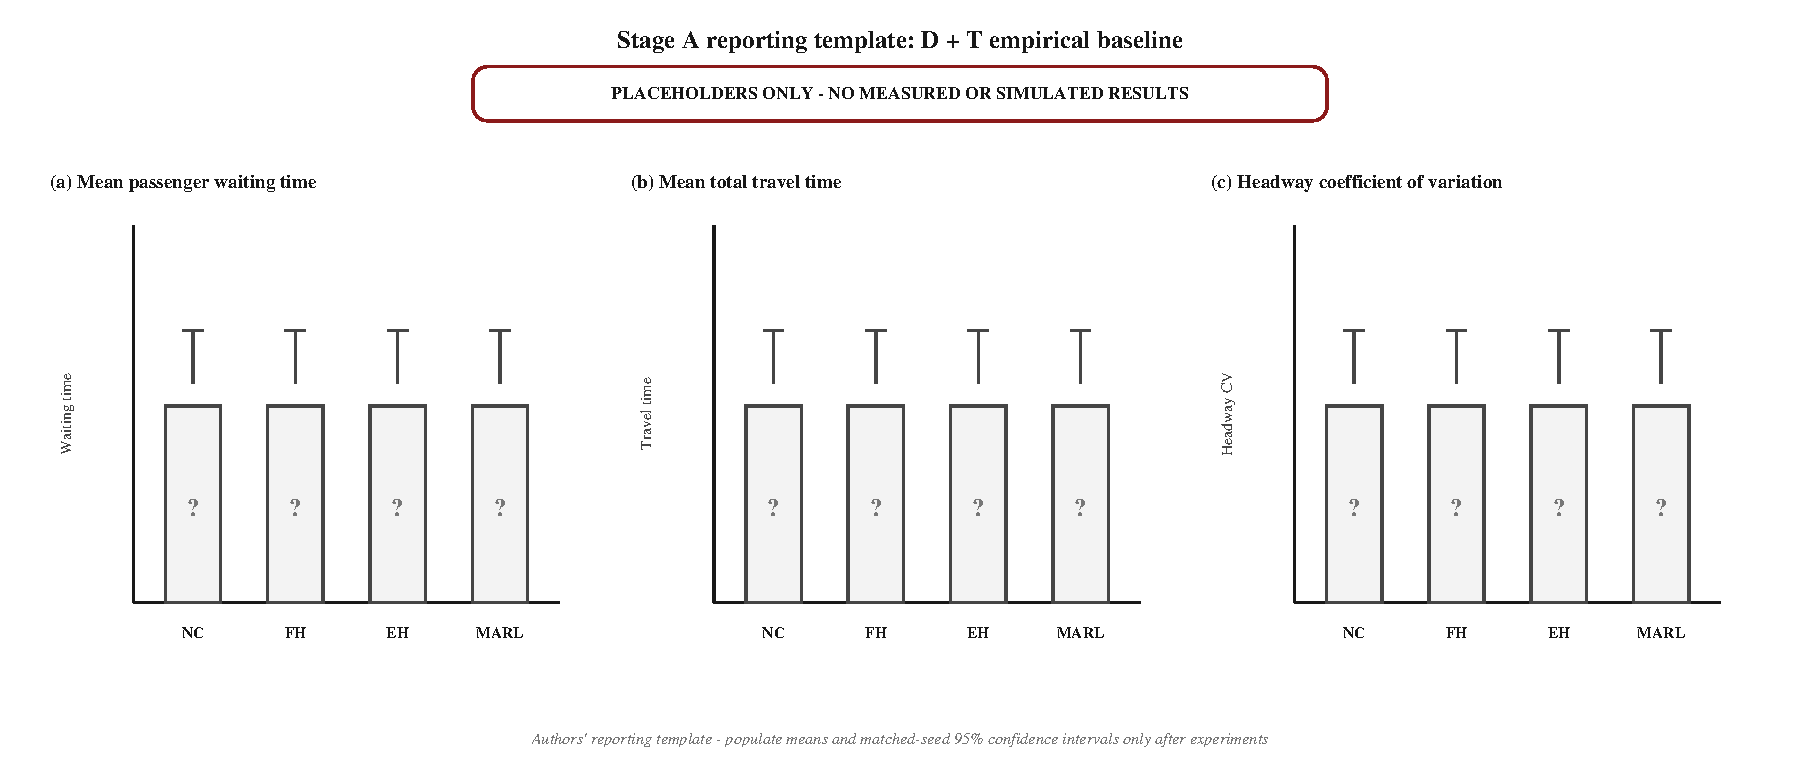
\includegraphics[width=0.8\textwidth]{Figures/meth_fig_eo3_1_ideal_results.pdf}
    \caption[Illustrative Stage A output format]{Illustrative Output of the Stage A
    ideal-condition evaluation output, comparing the four controllers (NC, FH, EH,
    MARL) across the three response variables: (a) mean passenger waiting time,
    (b) mean total travel time, and (c) headway coefficient of variation. Error
    bars represent 95\% confidence intervals over $N \geq 30$ Monte Carlo runs
    with matched seeds. Numerical values shown are illustrative and do not
    reflect measured results. Authors' illustration.}
    \label{fig:stage-a-illustrative}
\end{figure}

\textbf{Stage B: Non-ideal-condition evaluation.} The trained MARL policy and the three baselines are evaluated across the swept disturbance range $\eta \in \{0.3, 0.6, 1.0, 1.3\}$, with the breakdown generator active at each level, using the Monte Carlo evaluation procedure illustrated in Figure~\ref{fig:aec-eval}. For each $(\eta, \text{controller})$ cell, $N \geq 30$ Monte Carlo iterations are run with matched seeds. Reported outputs are: (a) mean waiting time, travel time, and headway CV as functions of $\eta$ for each controller; (b) percentage degradation at each $\eta$ relative to the controller's own ideal-condition result; (c) the disturbance level at which MARL's advantage over the best-performing baseline becomes statistically significant; and (d) the degradation slope, defined as the rate of waiting-time increase per unit increase in $\eta$, with smaller slopes indicating greater resilience. An ablation is also run with each disturbance enabled alone (demand-only, weather-only, breakdown-only) at $\eta = 1.0$ to attribute degradation to disturbance type.

\paragraph{Stage B acceptance criterion} The MARL policy is reported as performing well under disturbance if its mean waiting time stays below that of the best-performing baseline across the full sweep, with statistical significance under the same correction as Stage A.

\begin{figure}[htbp]
    \centering
    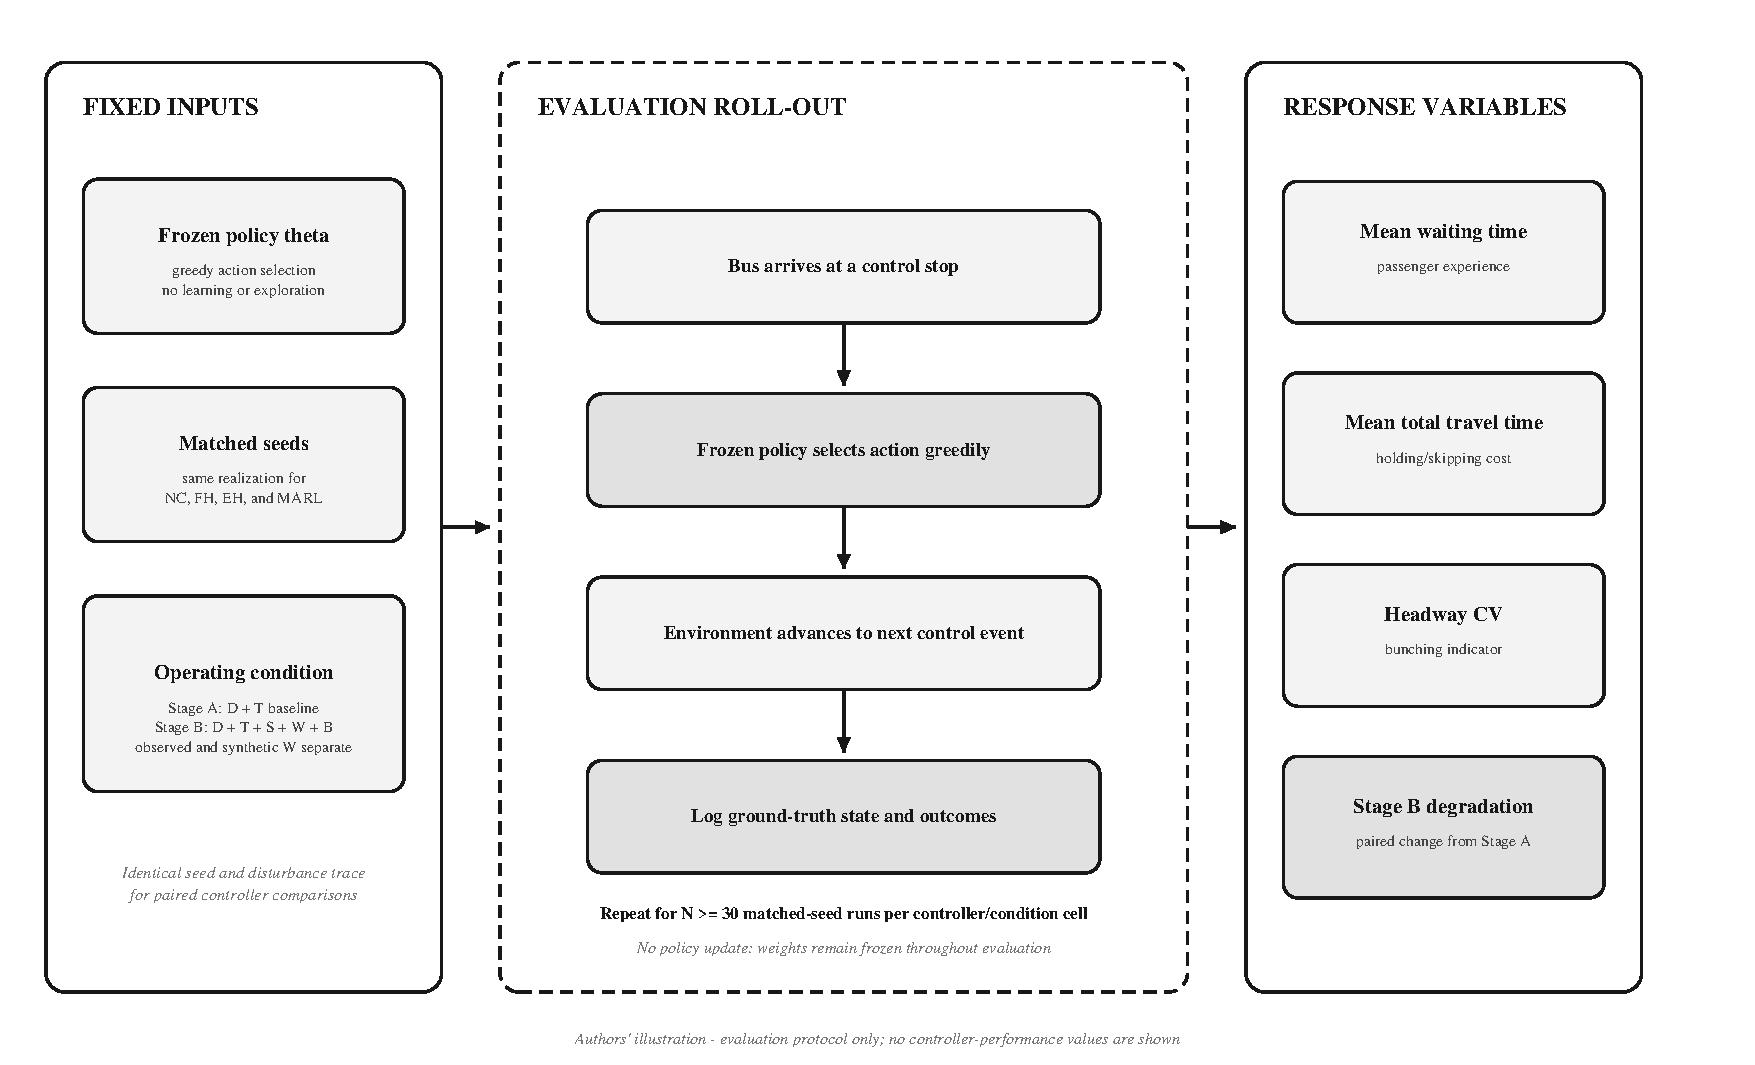
\includegraphics[width=1\textwidth]{Figures/fig_3_2b_aec_evaluation.pdf}
    \caption[Monte Carlo evaluation layer]{The Monte Carlo evaluation layer. The frozen policy $\theta$ selects the highest-valued action at each control stop without exploration or weight updates. Matched seeds ensure that every controller faces the same disturbance realization, so performance differences reflect the control strategy alone. Three response variables are recorded per run: mean passenger waiting time, mean total travel time, and headway coefficient of variation. Authors' illustration.}
    \label{fig:aec-eval}
\end{figure}


\section{Methodological Challenges}
\label{sec:challenges}

Three challenges shape the experimental design. The design is scoped to remain feasible on accessible hardware (a single cloud-notebook GPU runtime), and a tiered scope plan (stated at the end of this section) guarantees a defensible minimum deliverable even if the full sweep cannot be completed.

\textbf{Q-value overestimation under heavy-tailed returns.} Value-based methods such as DQN overestimate Q-values \cite{vanHasselt2016DDQN}, and this bias grows when returns are heavy-tailed, as they are under high-intensity disturbance \cite{Henderson2018Matters,Agarwal2021Precipice}. The DDQN double estimator addresses this by decoupling action selection from evaluation \cite{vanHasselt2016DDQN}. Because disturbances are active during training, reward clipping and target-network soft updates are used as additional stabilizers throughout, not only at the highest intensities.

\textbf{Computational cost.} The evaluation budget follows directly from the experimental factors. The full $\eta$ grid spans five values $\{0, 0.3, 0.6, 1.0, 1.3\}$, with $\eta = 0$ serving as the Stage A ideal condition and the remaining four levels constituting the Stage B non-ideal sweep. Stage A runs four controllers at $N \geq 30$ each, giving $4 \times 30 = 120$ runs. Stage B runs four controllers across four non-ideal levels at $N \geq 30$ per cell, giving $4 \times 4 \times 30 = 480$ runs. The single-disturbance ablation (Section~3.2.10) adds three conditions (demand-only, weather-only, breakdown-only) across the same four controllers at $N \geq 30$, giving $3 \times 4 \times 30 = 360$ runs, for a total of approximately 960 evaluation runs. Two decisions keep this tractable. First, SUMO is restricted to one-time calibration; all Monte Carlo runs execute in the lightweight Python environment. Second, evaluation runs are CPU-bound and parallelizable across random seeds, so training is the only phase requiring sustained GPU time.

\textbf{Timeline feasibility.} The full evaluation suite of approximately $960$ runs is expected to require on the order of single-digit hours of single-core CPU time, given the event-driven simulation rates reported in comparable work \cite{Wangsun,Rodriguez2023Cooperative}; parallelizing across seeds on a multi-core runtime fits the full sweep within a single working session. MARL training is sized to the episode budget reported by Rodriguez et al.~\cite{Rodriguez2023Cooperative}, who train for $500 + 300 = 800$ episodes in two phases. The total training budget, including hyperparameter tuning and reward-weight iteration (EO 2.1), is projected at approximately 30 hours of T4-class GPU time, which fits within standard cloud-notebook allocations without institutional HPC resources. These time figures are planning estimates to be confirmed empirically during implementation rather than measured values. A tiered scope plan is maintained: the minimum deliverable is Stage A ($\eta = 0$) plus a two-level non-ideal sweep at $\eta \in \{0.6, 1.0\}$; the full four-level non-ideal sweep and ablation series are added if calibration and training proceed on schedule.